\documentclass{article}

%Packages
\usepackage{amsmath}
\usepackage{amstext}
\usepackage{amssymb}
\usepackage{appendix}
\usepackage{coseoul}
\usepackage{enumerate}
\usepackage{graphicx}
\usepackage{import}
\usepackage{lscape}
\usepackage{modular}

\usepackage[pdfpagemode=UseNone,pdfstartview=FitH,colorlinks=true,linkcolor=blue,citecolor=blue,urlcolor=blue]{hyperref}
\usepackage[all]{hypcap}


% General physics constructs
\newcommand{\bra}[1]{\langle #1 |}
\newcommand{\ket}[1]{| #1 \rangle }
\newcommand{\braket}[2]{\langle #1|#2\rangle}
\newcommand{\bbraket}[3]{ \langle #1 | #2 | #3 \rangle }
\newcommand{\norm}[1]{\| #1\|}
\newcommand{\avg}[1]{\left \langle #1 \right \rangle}
\newcommand{\angavg}[1]{\left \langle #1 \right \rangle}
\newcommand{\abs}[1]{\left \lvert #1 \right \rvert}
\newcommand{\VS}{\textit{\textbf{V}}}
\newcommand{\Tr}{\textrm{Tr}}
\renewcommand{\Re}{\textrm{Re}}
\renewcommand{\Im}{\textrm{Im}}
\newcommand{\basis}[1]{\{\ket{#1}\}}

\newcommand{\omegaqubit}{\omega_{10}}

% Figures. Example usage:
% \quickfig{\columnwidth}{my_image}{This is the caption}{fig:my_fig}
\DeclareRobustCommand{\quickfig}[4]{
\begin{figure}
\begin{centering}
\includegraphics[width=#1]{#2}
\par\end{centering}
\caption{#3}
\label{#4}
\end{figure}
}

\DeclareRobustCommand{\quickwidefig}[4]{
\begin{figure*}[h]
\begin{centering}
\includegraphics[width=#1]{#2}
\par\end{centering}
\caption{#3}
\label{#4}
\end{figure*}
}


\begin{document}

\title{Random walk on a cube}
\author{Daniel Sank}
\date{Date: Some time in grad school}

\maketitle

This was originally written as a letter to Sasha Korotkov while we were trading hard problem back and forth over email.
This played a role in the somewhat unusual tone and tongue-in-cheek section headings, like ``5th grade''.

\section{The problem}

Suppose you start on a corner of a cube, and then make a random walk.
On each step, you go along an edge to one of the three neighboring vertices, each with probability $1/3$.
What is the mean number of steps you take before arriving at the diametrically opposed vertex \emph{for the first time}?

\section{Hint}

Note that from the symmetry of the problem there are four types of nodes: the starting node, three nodes that are one step from the start, three nodes that are two steps from the start, and the final node.
This is illustrated in Fig. \ref{Fig:cubeNetwork} a.
Because of the number of connections between nodes the problem can be reduced to a one dimensional network as shown in Fig. \ref{Fig:cubeNetwork} b.
This is a substantial simplification, but we still need to actually solve the problem.

\section{$5^{th}$ grade method}

Denote by $\langle A \rangle$ the mean number of steps it takes to get to $D$, starting from $A$. Define $\langle B \rangle$ and $\langle C \rangle$ similarly.
When we are at $A$, there is unity probability that we will step to $B$.
Mathematically, this is written
\begin{equation}
\langle A \rangle = 1 + \langle B \rangle \, .
\end{equation}
Similaraly, when we are at $B$ we can go to $A$ with probability $1/3$ or to $C$ with probability $2/3$.
In both cases, we add one step to $\langle C \rangle$ so we get
\begin{equation}
\langle B \rangle = \frac{1}{3}(1 + \langle A \rangle) + \frac{2}{3}(1 + \langle C \rangle) \, .
\end{equation}
By entirely similar reasoning you can write
\begin{equation}
\langle C \rangle = \frac{2}{3} (1 + \langle B \rangle) + \frac{1}{3} \, .
\end{equation}
Now you solve the system of linear equations to find $\langle A \rangle = 10$.

\begin{figure}
\begin{centering}
\includegraphics[width=10cm]{cubeNetwork.pdf} 
\par\end{centering}
\caption{The random walk on a cube. a) There are four types of nodes. b) The cube is equivalent to a line of nodes.}
\label{Fig:cubeNetwork}
\end{figure}


\section{High school method}

Think of the probability distribution over the points $A$, $B$, and $C$ as a column vector
\begin{equation}
\left[ \begin{matrix} P_A \\ P_B \\ P_C \end{matrix} \right] \, .
\end{equation}
With this picture, each step of the process can be represented by multipliction of a process matrix
\begin{equation}
T = \left[ \begin{matrix} 0 & 1/3 & 0 \\ 1 & 0 & 2/3 \\ 0 & 2/3 & 0 \end{matrix} \right] \, .
\end{equation}
For a given state $\ket{P}$, the probability that the process is still alive (has not been absorbed at $D$) is the sum of all entries in $\ket{P}$.
This can be written as $\braket{1}{P}$ where $\bra{1}$ corresponds to \begin{equation}
\left[ \begin{matrix} 1 & 1 & 1 \end{matrix} \right] \, .
\end{equation}
To find the mean number of steps before absorption, we just sum up the probabilities that the process is still alive at each step \begin{align*}
\langle A \rangle &= \sum_{n=0}^{\infty} \bra{1} T^n \ket{A} \\
&= \bra{1} \left( \sum_{n=0}^{\infty} T^n \right) \ket{A} \\
&= \bra{1} (1-T)^{-1} \ket{A} \\
&= 10 \, .
\end{align*}
Here we used the formula for the geometric series but applied it to matrices with no justification.
This is the beautiful way of the "physicist" but I think also the way of the really good mathematician.


\section{College method}

This is way I originally figured out to do the problem. I guess I'm not clever enough for the simple solutions.

First read the accompanying document on generating functions for first passage problems.

We take the process matrix for the completely unconstrained diffusion on the cube
\begin{equation}
T = \left[ \begin{matrix} 0 & 1/3 & 0 & 0 \\ 1 & 0 & 2/3 & 0 \\ 0 & 2/3 & 0 & 1 \\ 0 & 0 & 1/3 & 0\end{matrix} \right] \, .
\end{equation}
For a given starting state $\ket{i}$, the probability distribution $n$ steps later is
\begin{equation}
T^n \ket{i} \, .
\end{equation}
We can therefore easily compute the probability to be in state $\ket{j}$ after $n$ steps
\begin{equation}
p_{ji}(n) = \braket{j}{T^n | i} \, .
\end{equation}
This is not so hard to compute because $T$ is symmetric and can be diagonalized.
Once you have $p_{ji}(n)$ it is simple to compute $P_{ji}(z)$ by geometric series,
\begin{equation}
P_{ji}(z) = \sum_{n=0}^{\infty}z^n p_{ji}(n) \, .
\end{equation}
We then find $F_{ji}(z)$ according to $F_{ji}(z) = P_{ji}(z)/P_{jj}(z)$.
The mean first passage time is just
\begin{equation}
\lim_{z\rightarrow 1} \frac{d}{dz}F_{ji}(z) \, .
\end{equation}
If you're very careful about the lower limits on the sums you get the correct answer (I have not been careful in this document but I've worked it out carefully before).

One thing I found very interesting about this problem is that you get the right answer even though you use the geometric series formula, but then later take $z\rightarrow 1$, which is a case where the geometric series formula should not work.

\end{document}
